\section{Data}
    % Suggested 300 words

    \paragraph{Data provenance}
        We used two datasets to aid our investigation: an IMDB movie dataset, containing
            various details about movies made from 2006-2016; and a larger movie dataset (TMD),
            containing details about movies released on or before July 2017.
        The IMDB dataset has a bit of a contentious past as it was scraped off of the movie
            ranking website IMDB.com, and is actually only a sample dataset from a much larger
            dataset that has every movie made from 2006-2016 that is in the IMDB.
        The large movie dataset (TMD) was collated using data from TMDB (The Movie DataBase) and 
            grouplens.org; but we only use the part that was obtained from TMDB as it is used
            to find Director and Actor experience.

        Both datasets were downloaded from kaggle.com, a data science platform that enables users
            to access and share datasets. These datsets are shared underneath the CC0 1.0 Universal
            Public Domain Dedication, as such we will use them underneath fair use.

    \paragraph{Data description}
        The IMDB movie dataset has 12 columns, all either containing string values or floating point values.
        The only odd column is the Genre column which contains the different genres that can be applied to a particular movie.
        The genres that are in this dataset are the arbritary genres: 
            
        Action, Adventure, Sci-Fi, Mystery, Horror, Thriller, Animation, Comedy, Family, Fantasy, Drama, Music, Biography, Romance, History, Crime, Western, War, Musical, Sport
        
        The column summary is shown in Figure \ref*{fig-IMDB-Movie-Data-Column-Description}.
        \begin{figure}[h]
            \centering
            \begin{tabular}[width = \textwidth]{lll}
                \toprule
                Column Name &           Description                                                                 & Data Type \\
                \midrule
                Rank &                  The rank the movie has in the IMDB database                                 & Integer \\          
                Title &                 The name of the movie                                                       & String \\
                Genre &                 The genres that apply to the movie, there can be anywhere from              & Genre \\
                {}      &               1-3 genres. A genre can be any from: Action, Adventure, Sci-Fi,             & Category \\
                {}      &               Thriller, Animation, Comedy, Family, Fantasy, Drama, Music,                 & {} \\
                {}      &               Romance, History, Crime, Western, War, Musical, Sport, Horror               & {} \\
                {}      &               Mystery, Biography                                                          & {} \\
                Description &           The description of the movie                                                & String \\
                Director &              The person who directed the movie                                           & String \\
                Actors &                The lead roles in the movie                                                 & String \\
                Year  &                 The year the movie was released                                             & Integer \\
                Runtime (Minutes) &     The runtime in minutes of the movie                                         & Integer \\ 
                Rating   &              The mean rating of the movie, taken from IMDB.com                           & Float \\
                Votes   &               The amount of users that voted on a movie to give it that rating            & Integer \\ 
                Revenue (Millions) &    The gross income the movie made at the US box office                        & Float \\  
                Metascore   &           The rating of movie, determined using aggregated weighted Critics           & Integer \\
                {}          &           scores                                                                      & {} \\         
                \bottomrule
            \end{tabular}
            \caption[short]{The different columns in the IMDB-Movie-Data.csv file}\label{fig-IMDB-Movie-Data-Column-Description}
        \end{figure}
        \newline
        The TMD dataset used had a bit of a more odd structure.
        We only used the crew.csv file that is a small part of the larger dataset, so we only explain the structure of crew.csv.
        This file was composed of three columns: cast, crew and id.
        The odd part of the dataset is that the cast and crew columns are composed of .json files, and as such we needed to parse 
            out the useful data from these json files to actually get useable data.
        The column summary is shown in Figure \ref*{fig-Credits-Column-Description}.
        \begin{figure}[h]
            \centering
            \begin{tabular}[width = \textwidth]{lll}
                \toprule
                Column Name &           Description                                                                 & Data Type  \\
                \midrule
                cast &                  The cast list of the movie, including all actors who appeared in it.        & .json file \\          
                crew &                  The entire crew list of the movie, including all the people who made it.    & .json file \\
                id &                    The movie id. This is used in the larger dataset to connect data together   & Integer     \\        
                \bottomrule
            \end{tabular}
            \caption[short]{The different columns in the credits.csv file}\label{fig-Credits-Column-Description}
        \end{figure}

    \paragraph{Data processing}
        To cleanup the TMD dataset, we made and used a python script that went through all the entries of
            the dataset and extracted two things; number of movies each actor appeared in, and number of movies each director
            directed.
        These two sets of data were saved to .csv files, named actor\_counts.csv and director\_counts respectively.
        \\
        Using this newly acquired data, we merged it with the original IMDB dataset. 
        In the merging process the Description column was dropped, and the Director and Actor columns were replaced with the 
            Director Exp. and Mean Lead Roles Exp.
        This resulted in a merged\_movie\_data.csv file with structure shown in Figure \ref*{fig-merged-data-column-description}.
        \begin{figure}[h]
            \begin{tabular}[width = \textwidth]{lll}
                \toprule
                Column Name &           Description                                                                 & Data Type \\
                \midrule
                Rank &                  See fig \ref*{fig-IMDB-Movie-Data-Column-Description}                       & Integer \\          
                Title &                 See fig \ref*{fig-IMDB-Movie-Data-Column-Description}                       & String \\
                Genre &                 See fig \ref*{fig-IMDB-Movie-Data-Column-Description}                       & Genre \\
                Director Exp. &         The number of movies that the director of the movie has made                & Float \\
                Mean Lead Roles Exp. &  The mean number of movies that the lead actors have been in                 & Float \\
                Year  &                 See fig \ref*{fig-IMDB-Movie-Data-Column-Description}                       & Integer \\
                Runtime (Minutes) &     See fig \ref*{fig-IMDB-Movie-Data-Column-Description}                       & Integer \\ 
                Rating   &              See fig \ref*{fig-IMDB-Movie-Data-Column-Description}                       & Float \\
                Votes   &               See fig \ref*{fig-IMDB-Movie-Data-Column-Description}                       & Integer \\ 
                Revenue (Millions) &    See fig \ref*{fig-IMDB-Movie-Data-Column-Description}                       & Float \\  
                Metascore   &           See fig \ref*{fig-IMDB-Movie-Data-Column-Description}                       & Integer \\
                \bottomrule
            \end{tabular}
        \caption[short]{The different columns in the merged data set}\label{fig-merged-data-column-description}
        \end{figure}

        To check this data was properly normalised we made a histogram plot of all the numeric variables, shown in Figure \ref*{fig-distribution-of-numeric-variable}.
        As expected, a few variables did not appear to be normally distributed, namely: Revenue (Millions), Votes, Runtime (Minutes), 
            Director Exp., and Rating.
        \begin{figure}[h]
            \centering
            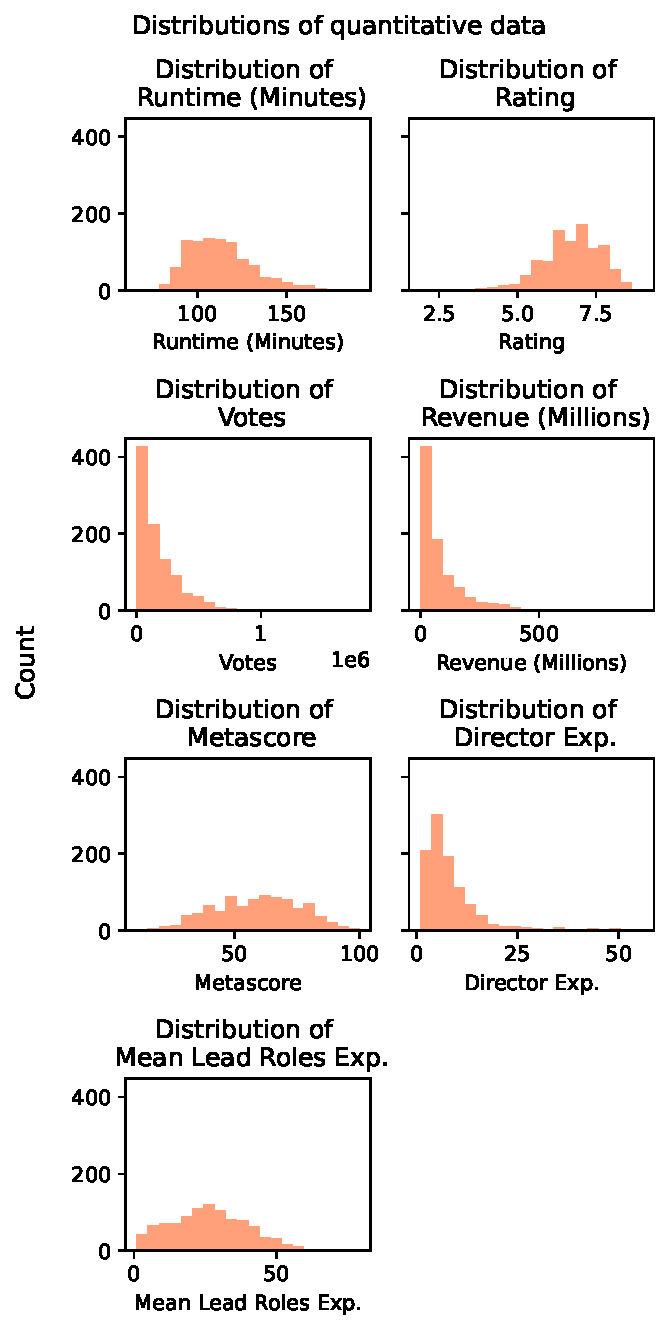
\includegraphics[width=0.8\linewidth]{Final/Distribution of Numeric Variables (No Transformation).pdf}
            \caption[short]{The distributions of the numeric variables in the merged dataset}\label{fig-distribution-of-numeric-variable}
        \end{figure}
        As shown in the plot, Revenue (Millions) and Votes are severly right skewed, implying an exponential distribution;
        Runtime (Minutes) and Director Exp. appear to be less severly right-skewed, implying a lognormal distribution;
        Rating seems to be left-skewed.
        The transformations for these variables that gave the best approximations to a normal distribution were:
        \begin{multicols}{2}
            \begin{itemize}
                \item Revenue (Millions) : Cube Root transform
                \item Votes              : Cube Root transform
                \item Runtime (Minutes)  : Log transform
                \item Director Exp.      : Log transform
                \item Rating             : Square transform
            \end{itemize}
        \end{multicols}
        Figure \ref*{fig-transformed-distribution-of-numeric-variable} shows the transformed and normalised numeric variables.
        The label has the p-values from testing whether the transformed distribution is normal, using the Kolmogorov-Smirnov
            test for goodness of fit.
        One interesting note is that altough the Director Exp. column fails the Kolmogorov-Smirnov test, there is clearly missing
            data; around 3 columns are missing from the histogram shown.
        With this in mind, and as the histogram does follow the normal distribution curve, there is sufficient evidence to assume
            ln(Director Exp.) has a normal distribution.
        \begin{figure}[h]
            \centering
            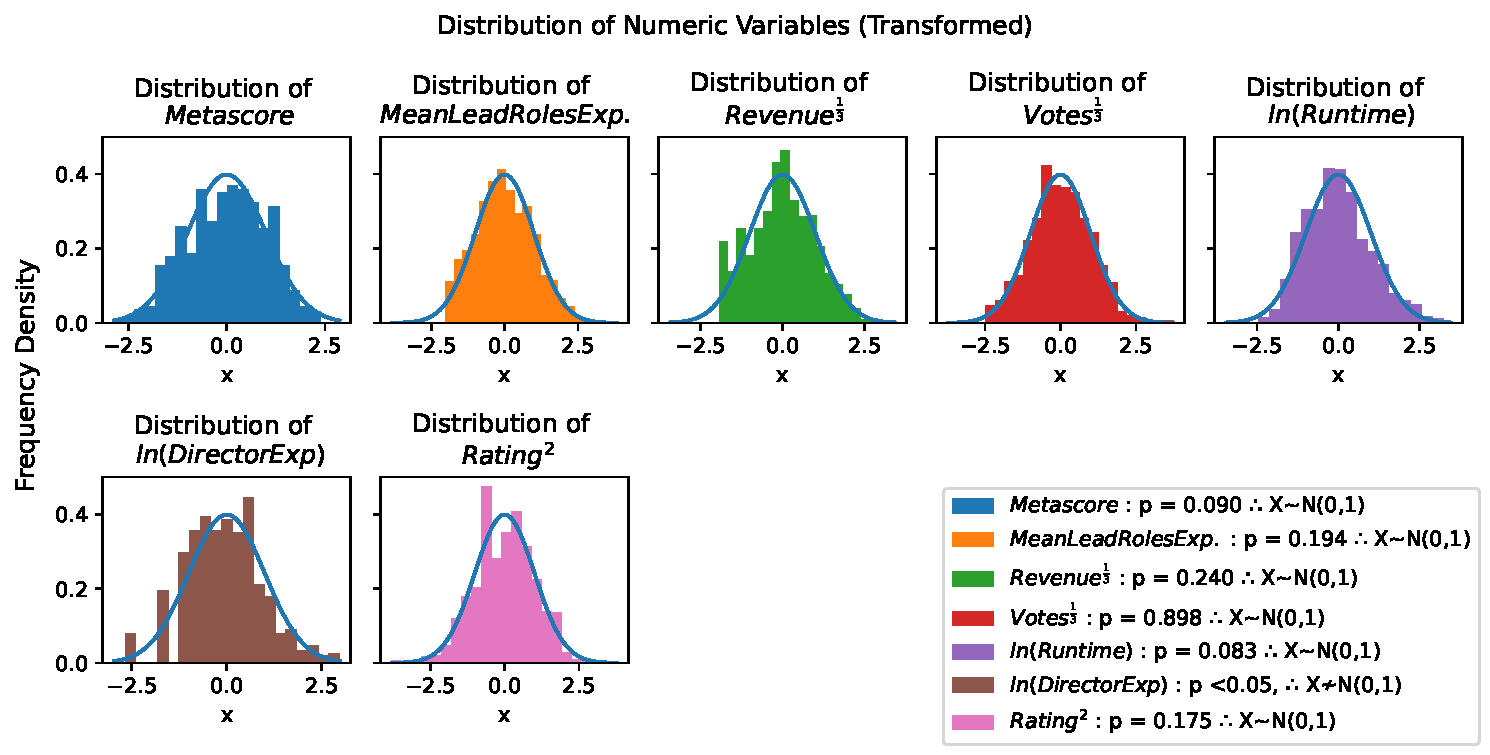
\includegraphics[width=\linewidth]{Final/Distribution of Numeric Variables (Transformed).pdf}
            \caption[short]{The distributions of the numeric variables in the merged dataset}\label{fig-transformed-distribution-of-numeric-variable}
        \end{figure}
        This normalised data was used for the rest of our investigations later on.
